% !TEX root = ../main.tex
\section{Maximum and Minimum Values of a Function}
	
\begin{figure}[h!]
	\centering
	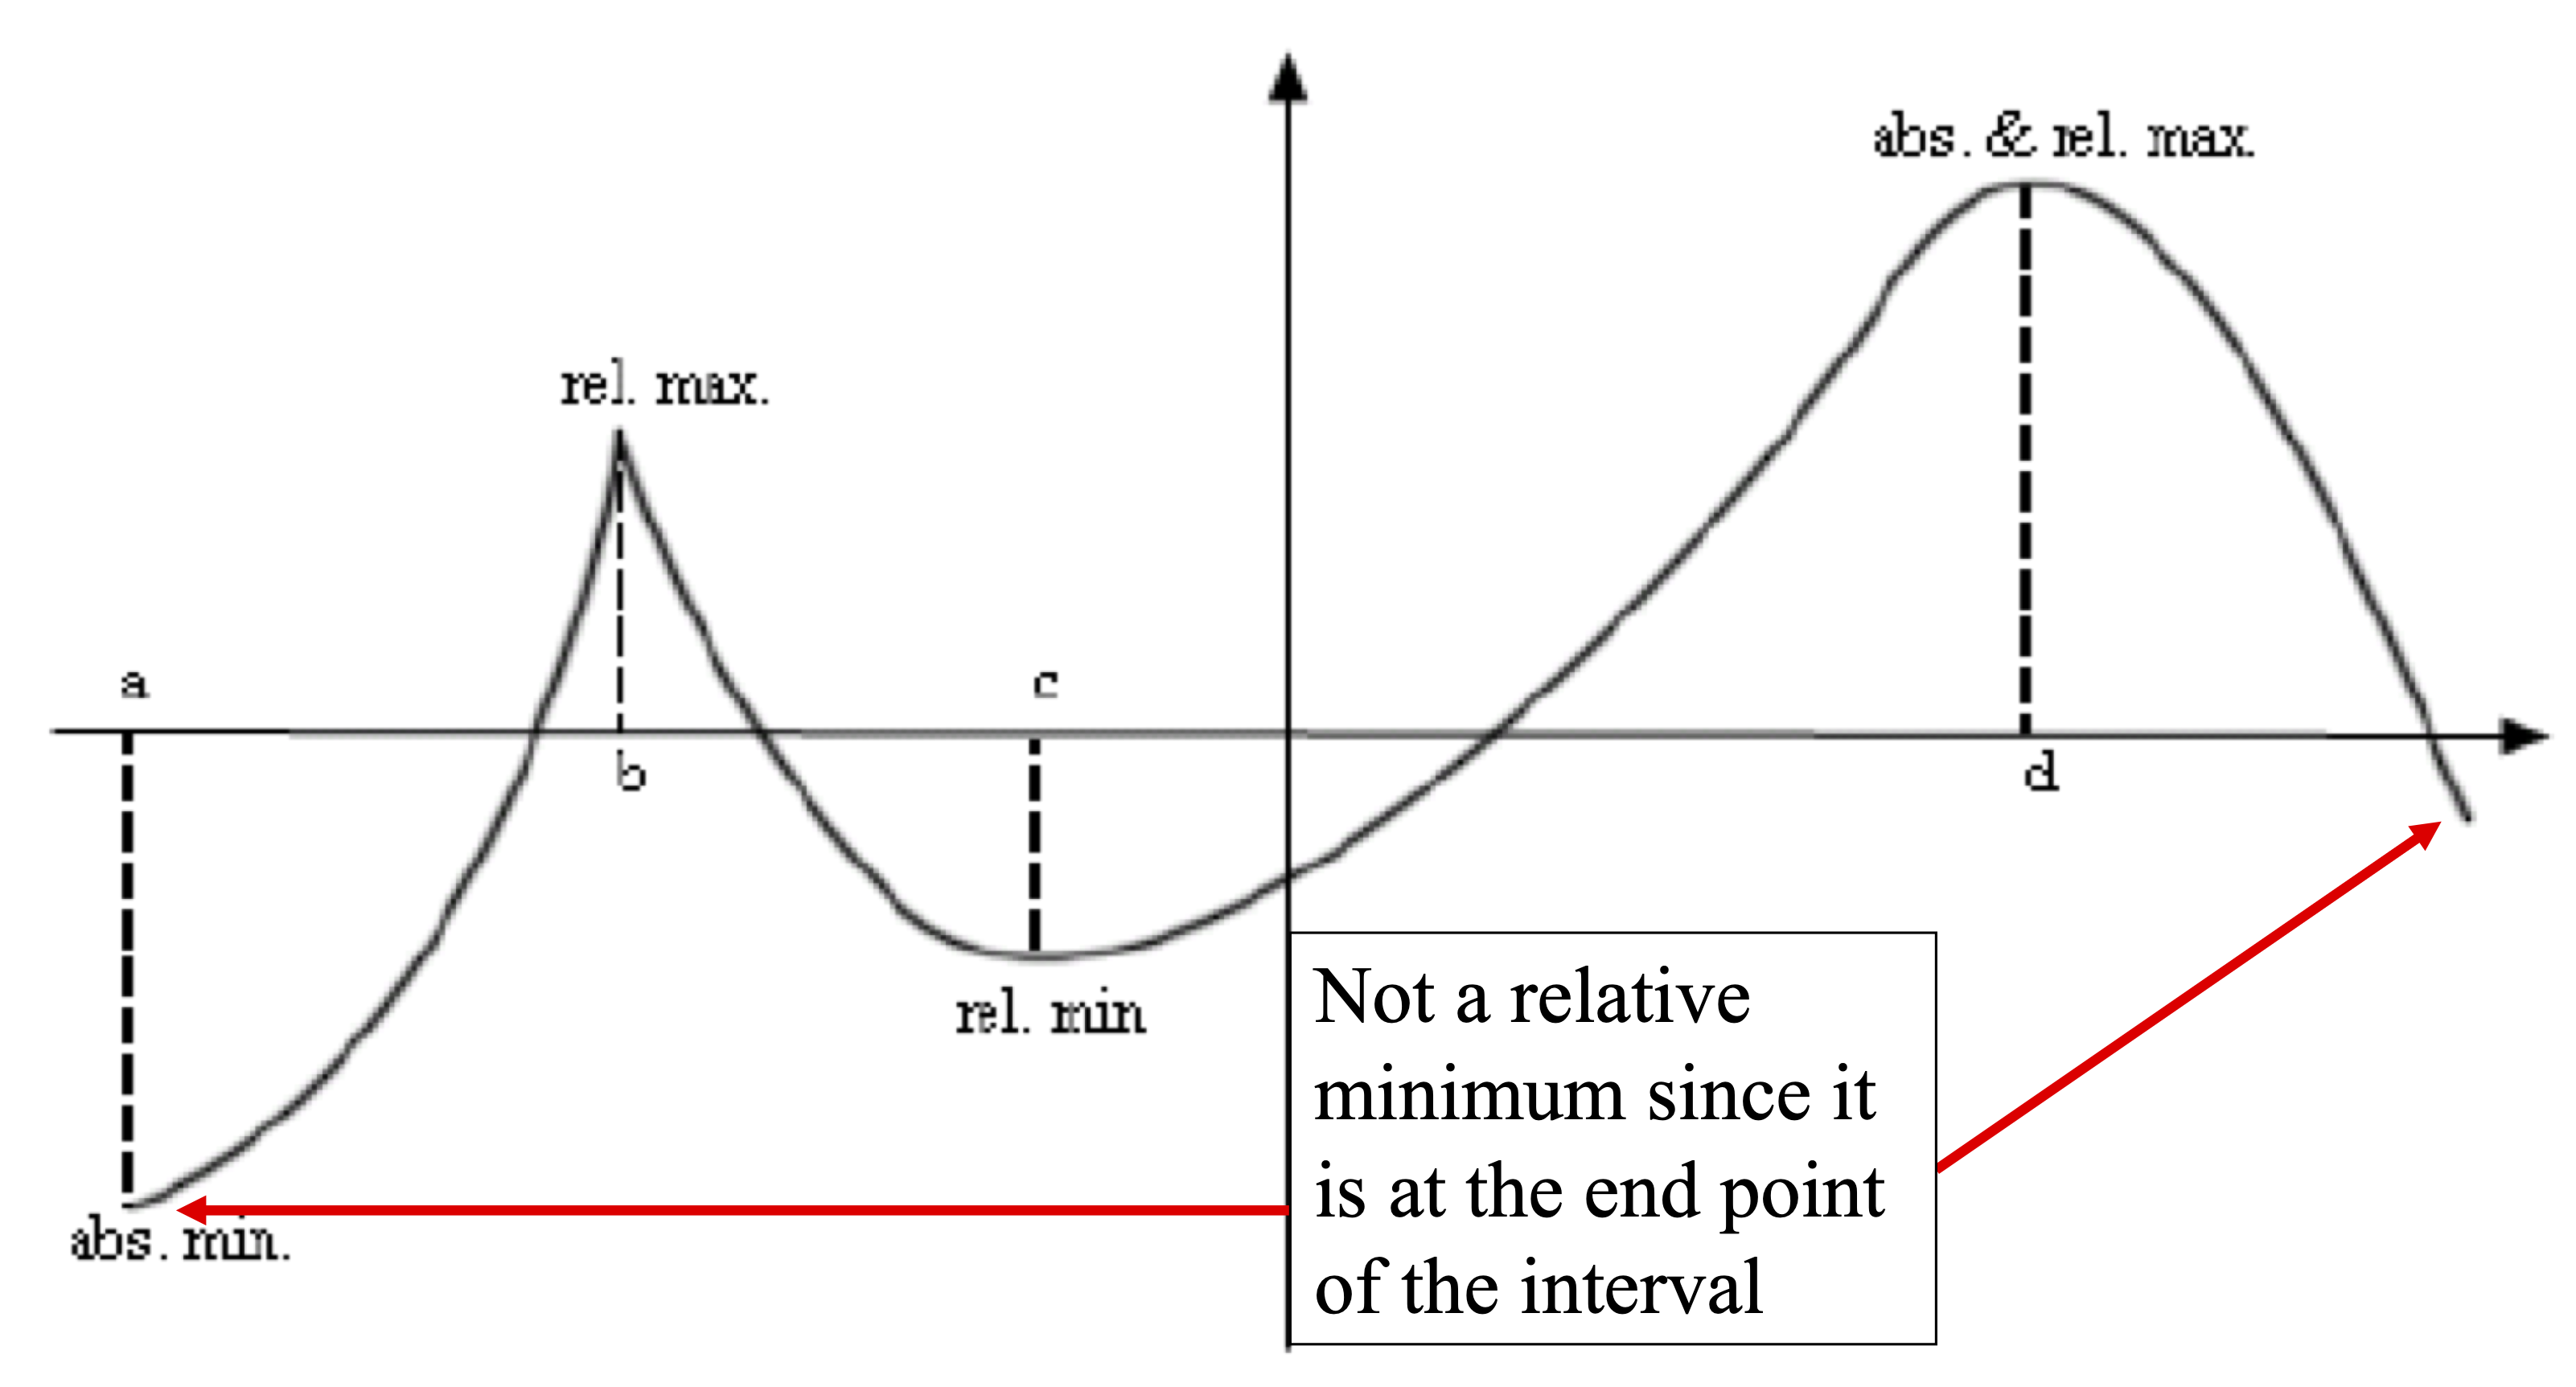
\includegraphics[width=0.9\linewidth]{chapter3/max-min}
	\caption{Maximum and minimum values.}
	\label{fig:max-min}
\end{figure}


\begin{myframe}[arc=10pt,auto outer arc]
	\begin{enumerate}
	\item \textbf{First Derivative test:} Suppose that $f$ is continuous at a critical number $x_0$.
	\begin{enumerate}
		\item  \textbf{Relative maximum} at $x_0$: $f'(x < x_0) > 0$ and $f'(x > x_0) < 0$
		\item  \textbf{Relative minimum} at $x_0$: $f'(x < x_0) < 0$ and $f'(x > x_0) > 0$
		\item  \textbf{No relative extremum} at $x_0$: No changes in sign of $f'(x_0)$
	\end{enumerate}
	
	
	\item \textbf{Second Derivative test:} Suppose that $f$ is twice differentiable $x_0$ and $f'(x_0)=0$.
		\begin{enumerate}
			\item \textbf{Relative minimum} at $x_0$: $f'' > 0$
			\item \textbf{Relative maximum} at $x_0$: $f'' < 0$
			\item \textbf{Inconclusive:} $f'' = 0$
    	\end{enumerate}
	
	\end{enumerate}
\end{myframe}

\newpage
\problem{Find the relative and absolute extremum values for $f(x)=2x^3-15x^2+36x$ on the interval $[1, 5]$.}

%%%% GUIDES
\qrfigure{chapter3/qr/Maximum-and-Minimum-Values}{Scan for guides}

